\clearpage
\addcontentsline{toc}{section}{References}
\begin{thebibliography}{99}

\addcontentsline{toc}{subsection}{\F}
\section*{\F}

\bibitem{kelly}
\href{http://www.amazon.com/FORTH-Text-Reference-Prentice-Hall-software/dp/0133263495}{amazon}
\emph{\F: A Text and Reference}\\
Mahlon G. Kelly, Nicholas Spies.

\addcontentsline{toc}{subsubsection}{in russian}
\subsection*{In russian}

\bibitem{cactus} \url{http://www.forth.org.ru/~cactus/library.htm}

\bibitem{kellyru}
\begin{tabular}{p{2cm} p{7cm}}
\raisebox{-0.9\totalheight}{
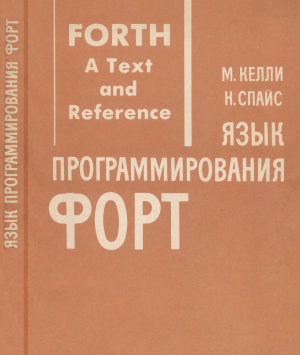
\includegraphics[width=2cm]{img/kelly_ru.jpg}}
% \end{minipage}
&
\href{http://www.forth.org.ru/~cactus/files/kelly.rar}{txt}
\emph{Язык программирования Форт}\par
М.Келли, Н.Спайс.\par
{\footnotesize Перевод с английского\par Е.В. Куркова, Ю.А. Семенова.}\par
{\small Москва, <<Радио и связь>>, 1993}\\
\end{tabular}

\bibitem{baranov}
\href{http://www.forth.org.ru/~cactus/files/baranov2.rar}{txt}
\emph{Язык Форт и его реализации}\\
С.Н. Баранов, Н.Р. Ноздрунов\\
{\small Лениград, <<Машиностроение>> Ленинградское отделение, 1988}


\end{thebibliography}